\subsection*{Redigering af brugeroplysninger} \label{sec:redigrering}
Brugeren har ud fra app'ens hovedmenu mulighed for at redigere adgangskode samt sygdomsspecifikke oplysninger. Af \autoref{fig:Redigerbrugeroplysninger} er aktivitetsdiagrammet for redigering af brugeroplysninger illustreret. 

\begin{figure}[H]
\centering
\textbf{Aktivitetsdiagram: Redigering af brugeroplysninger}\par\medskip
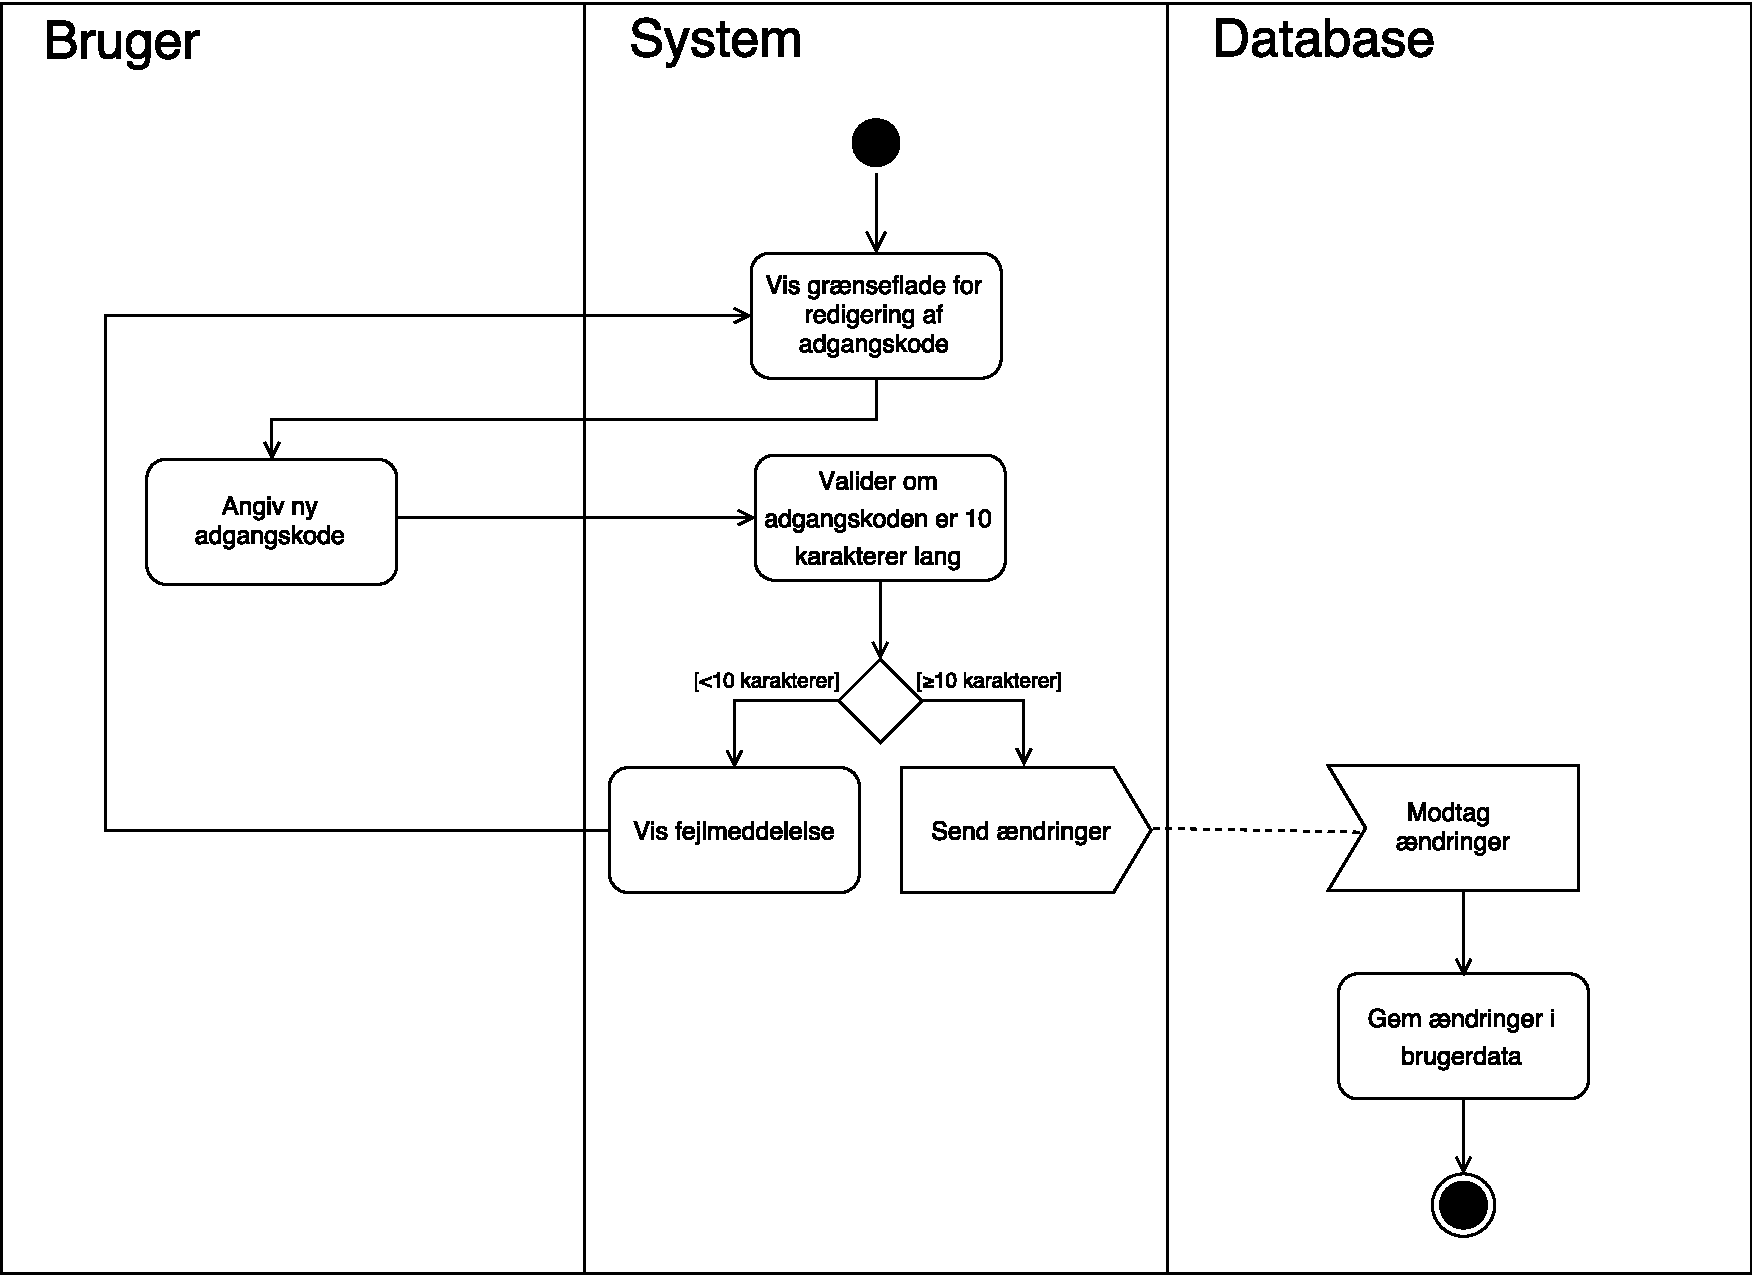
\includegraphics[width=0.9\textwidth]{figures/aktivitetsdiagram/Redigerbrugeroplysninger}
\caption{Aktivitetsdiagram for redigering af brugeroplysninger. Kategorisering af KOL uddybes af \autoref{fig:Kate}.}
\label{fig:Redigerbrugeroplysninger}
\end{figure}

\noindent
Det skal både være muligt at ændre sin adgangskode samt kategorisering, som blev defineret i forbindelse med registrering af brugeren. Da brugeren får tildelt en randomiseret adgangskode, skal det være muligt at ændre denne til en personlig adgangskode. For at kunne foretage en ændring af adgangskoden, skal den nye adgangskode som minimum være 10 karakterer lang. Grunden til dette er, at der ved log ind sendes en fejlmeddelelse, hvis indtastede informationer ikke findes i databasen, dertil skal adgangskoden ikke kunne forveksles med fejlmeddelelsen. Desuden anbefalder Rådet for Digital Sikkerhed, at adgangskoder bør være minimum 10 karakterer lang, dog er dette ikke et krav \citep{sikkerhed2015}.
Hvis kravet om minimum 10 karakterer ikke opfyldes, sendes en fejlmeddelelse tilbage til brugeren, hvortil en ny adgangskode skal indtastes. 
I tilfælde af, at brugerens tilstand ændres er det ligeledes muligt at redigere denne. Aktivitetsdiagrammet for kategorisering af KOL fremgår af \autoref{fig:Kate}.
Ved korrekt redigering af brugeroplysningerne sendes ændringerne til databasen, hvorefter de gemmes i databasen.